% Based on the answer by qubyte at 
% http://tex.stackexchange.com/questions/9767/whats-a-good-package-for-typesetting-quantum-circuits
\documentclass[12pt]{standalone}
\usepackage{tikz}

\usetikzlibrary{backgrounds}
% Dirac Kets
\newcommand{\ket}[1]{\ensuremath{\left|#1\right\rangle}}

\begin{document}
    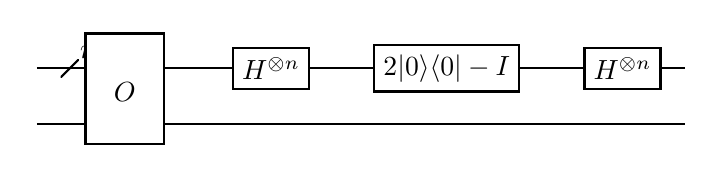
\begin{tikzpicture}[thick,
    cross/.style={path picture={ 
      \draw[black]
      (path picture bounding box.south) -- (path picture bounding box.north);
    }},
    swap/.style={path picture={ 
      \draw[black]
       (path picture bounding box.south west) -- (path picture bounding box.north east) 
       (path picture bounding box.south east) -- (path picture bounding box.north west);
    }},
    bundle/.style={path picture={ 
      \draw[black]
      (path picture bounding box.south west) -- (path picture bounding box.north east);
    }}]

    % `operator' will only be used by most gates.
    % `cnot' will refer to CNOT gates.
    % `phase' is used for controlled gates.
    \tikzstyle{operator} = [draw,fill=white,minimum size=1.5em]
    \tikzstyle{cnot} = [draw,cross,circle,minimum size=5pt]
    \tikzstyle{phase} = [draw,fill,shape=circle,minimum size=5pt,inner sep=0pt]
    %
    \matrix[row sep=0.4cm, column sep=0.8cm] (circuit) {

    % First row.
    \coordinate (start1); &[-0.5cm] 
    \node[bundle] (B0) {}; 
    \node[above right] (B0) {$n$}; &
    &
    \node[operator] (O12) {$H^{\otimes n}$}; 
    &
    \node[operator] (O13) {$2|0\rangle\langle 0| - I$};
    & 
    \node[operator] (O14) {$H^{\otimes n}$}; 
    &[-0.5cm]
    \coordinate (end1);\\
    
    % Second row.
    \coordinate (start2); &[-0.5cm] 
     &
     &
     &
     &
     &[-0.5cm]
    \coordinate (end2);\\
    };
    \draw [thick,black,fill=white] (-3.5,-2.3em) rectangle (-2.5,1.7em);
    \node at (-3,-0.15) (O) {$O$};

    \begin{pgfonlayer}{background}
        % Draw lines.
        \draw[thick] (start1) -- (end1) (start2) -- (end2) 
                     ;
    \end{pgfonlayer}
    %
    \end{tikzpicture}
\end{document}
